\chapter[Introduction]{Fundamentals of Statistical Signal Processing}

Statistical signal processing refers to the act of inferring generalizations from empirical data, with varying degrees of certainty.
In this introduction, we provide a unified view of detection and estimation theory.
The statistical problem we wish to explore can be described as follows.
We are interested in an unknown \emph{parameter} (or \emph{phenomenon}) which we denote by $\theta$.
We have access to an observation $Y$ that provides partial information about the value of $\theta$.
The connection between $Y$ and $\theta$ is probabilistic in nature, rather than explicit.
In particular, different values of $\theta$ may produce the same observation.
This abstract framework is illustrated below.

\begin{center}
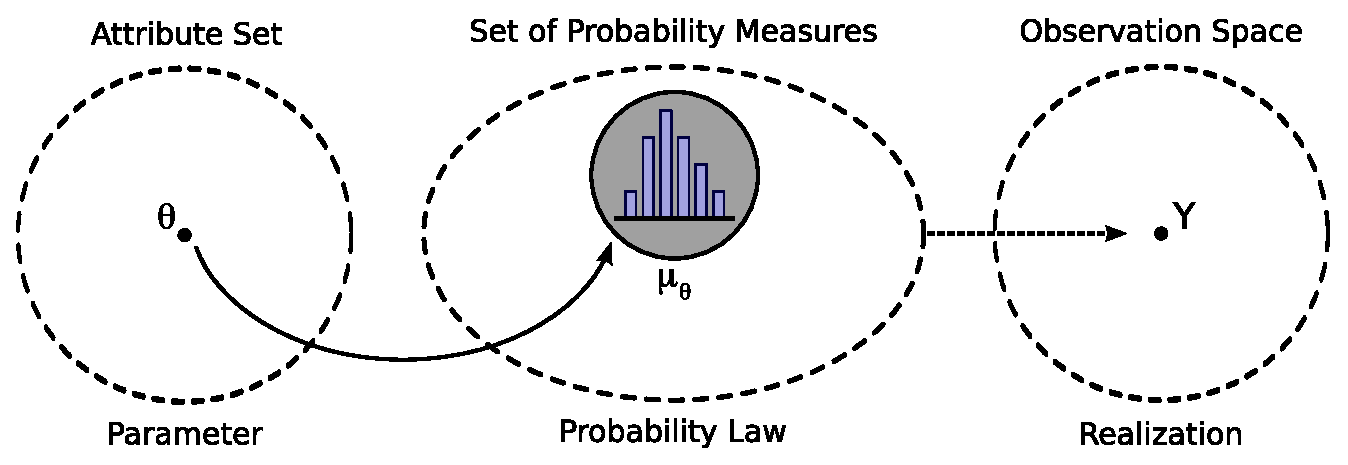
\includegraphics[width=5in]{Figures/1Chapter/Inference}
\end{center}

Three basic components are involved in this framework.
First, there is the \emph{attribute set} which is composed of all admissible values of $\theta$.
This set is represented by $U$.
The second component is a measurable space $(\mathcal{F}, \Omega)$ where $\Omega$ symbolizes the \emph{sample space} and $\mathcal{F}$ is the $\sigma$-algebra of all probability events.
Together, $\mathcal{F}$ and $\Omega$ provides a mathematical basis for the randomness induced by parameter $\theta$.
Finally, the \emph{observation space} $\Gamma$ is the collection of all realizable observations.
One obtains information about the true parameter $\theta$ by observing a random variable $Y$, which maps outcomes from the sample space $\Gamma$ to values in $\Gamma$.

If the attribute set contains a unique element, then the inference problem is trivial and we need not observe $Y$ to determine the value of $\theta$.
The more interesting case, of course, occurs when $U$ contains several distinct elements.
In this situation, the connection between $\theta$ and $Y$ becomes instrumental.
We explore this relationship next.

To each element $\theta \in U$, there corresponds a probability law $\mu_{\theta}$ acting on the measurable space $(\mathcal{F}, \Omega)$.
The true value of $\theta$ thus determines the distribution of random variable $Y$.
While observing the realization of $Y$ may provide information about its distribution, this empirical data is typically insufficient to resolve all the uncertainty surrounding the value of $\theta$.
Statistical signal processing broadly refers to the collection of techniques and methods employed to extract information about the phenomenon of interest from the available data.

\begin{center}
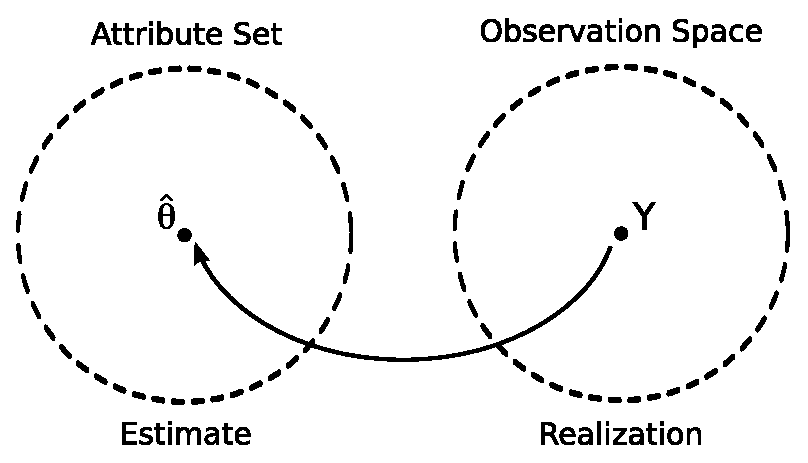
\includegraphics[width=3in]{Figures/1Chapter/StatisticalSignalProcessing}
\end{center}

We provide a simple example below to illustrate how this framework applies to engineering problems.

\begin{example} \label{example:BinaryCommunicationSystem}
A digital communication system transmits a single bit over a noisy channel, using a zero or a one.
The received information is corrupted by additive Gaussian noise, with distribution $\mathcal{N}(0,1)$.
We wish to decide which bit was sent from the received information.
To initiate this process, we cast this problem in the abstract framework described above.
In the present case, the attribute set is $U = \{ 0, 1 \}$; the sample space is the real line; and the corresponding probability density functions are
\begin{equation*}
f_0 (y) = \frac{1}{\sqrt{2 \pi}} e^{- \frac{y^2}{2}} \quad
f_1 (y) = \frac{1}{\sqrt{2 \pi}} e^{- \frac{(y-1)^2}{2}} .
\end{equation*}
Note that in this first example the observation space and the sample space are identical.
\end{example}

The primary characteristics that distinguish statistical inference problems from one another are the amount of a priori knowledge available about the attribute set $U$, the goal underlying the inference procedure, and the performance criterion used to assess the effectiveness of the inference procedure.
If the attribute set is partitioned into a finite or countable number of subsets and the objective is to identify which subset $\theta$ belongs to, then the decision process is termed \emph{detection} or \emph{hypothesis testing}.
In particular, a detector maps every element in the observation space $\Gamma$ to one of the admissible hypotheses.
A graphical interpretation of a detection process is illustrated below.

\begin{center}
\includegraphics[width=3in]{Figures/1Chapter/DetectionModel}
\end{center}

On the other hand, if $U$ contains an uncountable number of candidates and we are tasked with selecting the most appropriate one, then we are facing an \emph{estimation} problem.
In this setting, the goal is to select an estimate $\hat{\theta}$ based on observation $Y$ as to optimize a given objective function.
Thus, parameter estimation is a procedure that takes an argument in observation space $\Gamma$ and returns an element in the attribute set $U$.
The distinction between detection and estimation is at times rhetorical;
we will not delve on this issue.
Rather, our focus will be to develop a solid understanding of statistical signal processing and to become well-versed in applying some of its techniques and algorithms.

A second important distinction among inference problems, as mentioned above, comes from the assumptions made on attribute set $U$.
In \emph{classical estimation}, $U$ is taken to be a specific set containing the unknown parameter $\theta$.
This can be contrasted with the \emph{Bayesian approach} where $U$ is assumed to be a probability space with a specific distribution.
In this latter case, the value of $\theta$ is itself the outcome of a random experiment.
The distinction between these two approaches leads to disparate performance criteria, and hence different estimators.
Such a distinction is also present in detection problems, where the attribute set is either a collection of object with a deterministic parameter $\theta$, or a measurable space with a certain probability law.

A final and less straightforward distinction between inference problems stems from the nature of the empirical observations.
The framework detailed above implicitly assumes that observations can be viewed as random variables.
If on the other hand we have access to empirical data coming from a random process, then the inference problem becomes more challenging.
In this scenario, inference problems are referred to as \emph{signal detection} and \emph{signal estimation}.
When dealing with the progressive estimation of a stochastic process, the statistical inference procedure is often called \emph{filtering}.
We will address some of these problems once we acquire the mathematical sophistication necessary to tackle them.


\section{Modeling Engineering Problems}

These notes present a collection of important tools and methods in statistical signal processing.
Becoming familiar with these tools should provide the reader with the ability to solve various inference problems, and to assess the performance of the corresponding statistical procedures.
Still, an equally important skill to develop is the capacity to take a concrete engineering problem and to formulate it mathematically in a way that leads to a meaningful solution.
In this exposition, we will often use an abstract problem formulation as our starting point.
However, the value of being able to take an engineering challenge and to cast it in a relevant yet solvable framework is not to be understated.
Developing this skill is partly what sets apart the value of one's education and experience.
Throughout, we will provide examples and case studies of meaningful problems together with suitable mathematical interpretations.
Reading there examples carefully and understanding the process of selecting the proper tools to solve them should help develop good intuition.
While going through these notes, one should also try to think about new situations where the statistical methods under consideration apply.



%\section{Organization}
%
%These notes are organized as follows.
%
%In Chapter~\ref{chapter:Detection}, we study hypothesis testing.
%We begin with an introduction to the simplest such problem, binary detection.
%Both the classical and Bayesian forms of the problem are considered.
%The theory of detection is then extended to composite hypothesis testing, a framework where the attribute set contains more than two elements.
%We also discuss the problem of robust detection, sequential detection and quickest change detection.
%Finally, we look at simple instances of $M$-ary hypothesis testing.

%Chapter~\ref{chapter:ClassicalParameterEstimation} is devoted to classical parameter estimation.
%We first introduce the celebrated Cramer-Rao lower bound, which provides a performance limit on unbiased estimators.
%We then present the concept of sufficient statistics.
%This is followed by a discussion of common estimators including the best linear unbiased estimator, the maximum likelihood estimator, and the least squares estimator.
%The expectation-maximization algorithm is also introduced as a numerically tractable estimation methodology.
%
%Chapter~\ref{chapter:BayesianParameterEstimation} presents a study of Bayesian parameter estimation.
%The maximum a posteriori estimator is first introduced.
%This is followed by a discussion of the minimum mean square error and linear minimum mean square error estimators.
%Signal estimation is treated in Chapter~\ref{chapter:SignalEstimation}, where the Kalman-Bucy filter and the Wiener-Kolmogorov filter are introduced.

%estimating the median of a number of integers to which you only have a few observations.



